\documentclass[10pt,a4paper,twocolumn]{article}

\usepackage[T1]{fontenc}
\usepackage[utf8]{inputenc}
\usepackage{lmodern}
\usepackage{geometry}
\usepackage{microtype}
\usepackage{xcolor}
\usepackage{booktabs}
\usepackage{tabularx}
\usepackage{array}
\usepackage{listings}
\usepackage{caption}
\usepackage{float}
\usepackage{balance}
\usepackage{tikz}
\usetikzlibrary{arrows.meta,positioning,fit}
\usepackage{hyperref}
\usepackage{fancyhdr}
\usepackage{titlesec}

\geometry{
  top=19mm,
  bottom=20mm,
  left=18mm,
  right=18mm,
  columnsep=7mm
}

\hypersetup{
  colorlinks=true,
  linkcolor=blue!45!black,
  urlcolor=blue!55!black,
  pdftitle={DISTORT: Kubernetes-Native Disaggregated NVMe Storage over RDMA},
  pdfsubject={Technical project report},
  pdfkeywords={Kubernetes, CSI, NVMe-oF, RDMA, SPDK, disaggregated storage}
}

\definecolor{distortblue}{HTML}{173F5F}
\definecolor{distortcyan}{HTML}{007F86}
\definecolor{distortgreen}{HTML}{287D3C}
\definecolor{distortgray}{HTML}{F2F4F7}

\titleformat{\section}
  {\large\bfseries\color{distortblue}}
  {\thesection}{0.55em}{}
\titleformat{\subsection}
  {\normalsize\bfseries\color{distortcyan}}
  {\thesubsection}{0.5em}{}
\titlespacing*{\section}{0pt}{1.25em}{0.55em}
\titlespacing*{\subsection}{0pt}{0.95em}{0.35em}

\pagestyle{fancy}
\fancyhf{}
\lhead{\textsc{DISTORT Technical Report}}
\rhead{\thepage}
\renewcommand{\headrulewidth}{0.35pt}
\setlength{\headheight}{13.6pt}

\setlength{\parindent}{1em}
\setlength{\parskip}{0pt}
\renewcommand{\arraystretch}{1.15}
\newcolumntype{L}[1]{>{\raggedright\arraybackslash}p{#1}}

\lstset{
  basicstyle=\ttfamily\footnotesize,
  backgroundcolor=\color{distortgray},
  frame=single,
  rulecolor=\color{black!15},
  breaklines=true,
  columns=fullflexible,
  keepspaces=true,
  showstringspaces=false
}

\newcommand{\distort}{DISTORT}
\newcommand{\code}[1]{\texttt{\detokenize{#1}}}

\title{
  \vspace{-1.1cm}
  \textbf{\color{distortblue}\LARGE DISTORT}\\[0.25em]
  \Large Kubernetes-Native Disaggregated NVMe Storage over RDMA\\[0.35em]
  \normalsize Design, Implementation, and Preliminary Performance
}
\author{Technical Project Report}
\date{Implementation snapshot: 30 July 2026}

\begin{document}

\twocolumn[
\begin{@twocolumnfalse}
\maketitle
\vspace{-1.3em}
\end{@twocolumnfalse}
]

\section*{Introduction}

\distort{} (\textbf{DIS}aggregated \textbf{ST}orage \textbf{O}ver
\textbf{R}DMA \textbf{T}ransport) is a Kubernetes-native system for exposing
physical NVMe capacity from storage-provider nodes to workloads elsewhere in
the cluster. It connects Kubernetes Persistent Volume Claims (PVCs) to
NVMe-over-Fabrics (NVMe-oF) targets transported over RDMA. A workload receives
a normal Linux block device and filesystem even though the physical drive is
attached to another machine.

The system combines a declarative Kubernetes control plane with a direct
storage data path. Kubernetes objects, controllers, and CSI services decide
which device provides a volume and configure its export. Once the connection
is active, application I/O does not pass through the Kubernetes API, the
\distort{} manager, or the CSI controller. It travels from the consumer node's
filesystem and NVMe initiator, across the RDMA fabric, to either a Linux-kernel
or SPDK target on the provider and finally to the physical NVMe device.

This report describes the repository at commit
\code{bf92a29345d890c6aa1587af94c4feef3b4f5cbc}, including its API types,
controllers, node agent, CSI implementation, Helm chart, tests, and internal
project guide. It distinguishes implemented behavior from architectural intent
and future work. References to project ``novelty'' mean distinctive engineering
choices within \distort{}; a formal research-novelty claim would require a
separate systematic comparison with published systems.

\section{Design}

\subsection{Objectives and system boundaries}

\distort{} addresses the gap between Kubernetes' portable PVC model and the
host-local, privileged nature of NVMe hardware. A storage system must discover
controllers, decide which drives it is allowed to use, allocate capacity,
configure a fabric target, publish an endpoint, connect from the consumer, and
clean up state across several independently failing processes. \distort{}
represents these decisions in Kubernetes rather than hiding them behind a
single opaque storage service.

The design has four central objectives. First, a standard PVC should drive the
volume lifecycle through CSI. Second, discovering a device should not
automatically authorize destructive use; an administrator must explicitly
claim it. Third, Kubernetes should configure but not carry application I/O.
Fourth, the same control plane should support both kernel and user-space target
implementations.

The current system is not replicated storage. A volume has one provider and no
built-in mirroring, failover, or multipath. Snapshots, online expansion,
per-volume QoS, encryption, target authentication, and multi-tenant fabric
isolation are not implemented in the inspected snapshot. Placement is based on
available capacity rather than workload topology, provider health, failure
domains, or NUMA locality. These boundaries are important when comparing
\distort{} with a complete distributed storage platform.

\subsection{Control plane and data path}

The control plane contains the Kubernetes API, four custom resources, the
\distort{} manager and agent, the CSI driver, and Kubernetes CSI sidecars.
These components converge asynchronously. A CSI request creates desired state;
the manager assigns hardware; the provider agent configures the device and
target; and the completed endpoint returns through resource status.

The data path begins after the consumer stages the volume. For the SPDK
backend, the path is the application, mounted filesystem, Linux NVMe
initiator, InfiniBand/RDMA network, SPDK \code{nvmf_tgt}, SPDK logical volume,
and physical NVMe drive. The kernel backend follows the same consumer path but
terminates at Linux \code{nvmet} and a physical disk partition. A manager or
API outage therefore need not interrupt an established connection, whereas a
target, fabric, connection, or device failure can interrupt I/O.

\begin{figure*}[t]
\centering
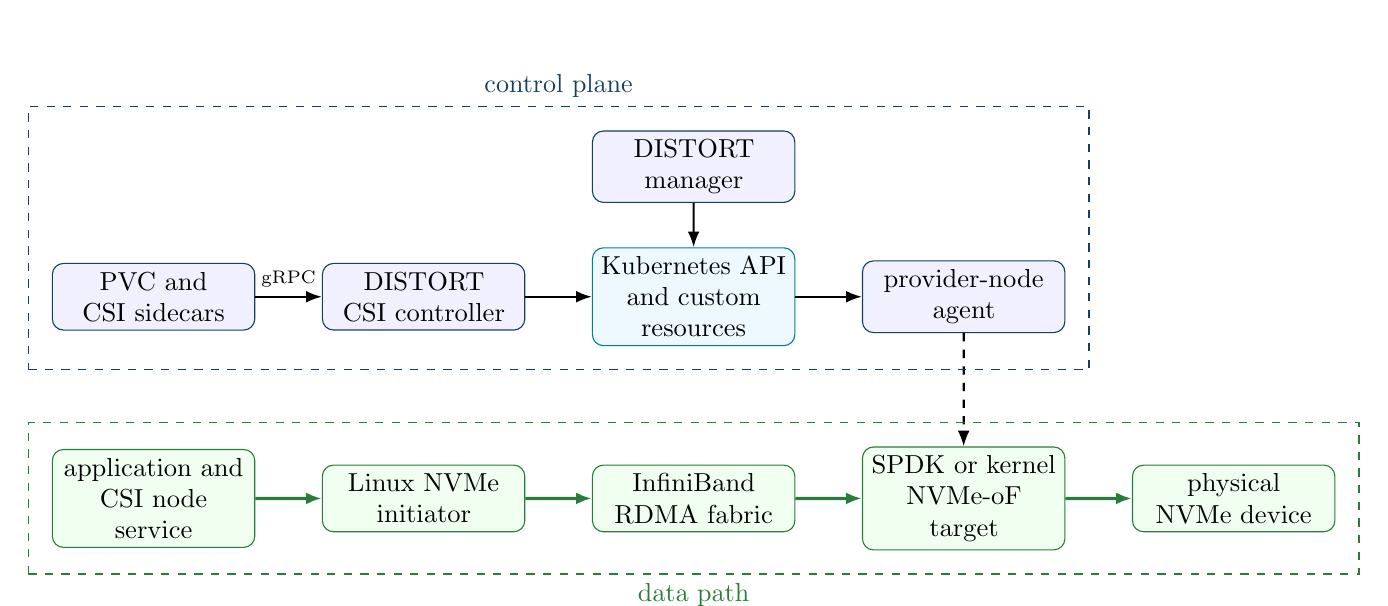
\begin{tikzpicture}[
  scale=0.94,
  every node/.style={transform shape},
  node distance=7mm and 9mm,
  box/.style={draw, rounded corners, align=center, minimum height=9mm,
              text width=25mm, fill=distortgray},
  ctrl/.style={box, draw=distortblue, fill=blue!6},
  data/.style={box, draw=distortgreen, fill=green!6},
  state/.style={box, draw=distortcyan, fill=cyan!7},
  arrow/.style={-{Latex[length=2mm]}, thick},
  io/.style={-{Latex[length=2mm]}, very thick, draw=distortgreen}
]
  \node[ctrl] (pvc) {PVC and\\CSI sidecars};
  \node[ctrl, right=of pvc] (csi) {\distort{}\\CSI controller};
  \node[state, right=of csi] (api) {Kubernetes API\\and custom resources};
  \node[ctrl, above=6mm of api] (manager) {\distort{}\\manager};
  \node[ctrl, right=of api] (agent) {provider-node\\agent};
  \node[data, below=16mm of pvc] (app) {application and\\CSI node service};
  \node[data, right=of app] (init) {Linux NVMe\\initiator};
  \node[data, right=of init] (fabric) {InfiniBand\\RDMA fabric};
  \node[data, right=of fabric] (target) {SPDK or kernel\\NVMe-oF target};
  \node[data, right=of target] (disk) {physical\\NVMe device};

  \draw[arrow] (pvc) -- node[above, font=\scriptsize]{gRPC} (csi);
  \draw[arrow] (csi) -- (api);
  \draw[arrow] (manager) -- (api);
  \draw[arrow] (api) -- (agent);
  \draw[arrow, dashed] (agent) -- (target);
  \draw[io] (app) -- (init);
  \draw[io] (init) -- (fabric);
  \draw[io] (fabric) -- (target);
  \draw[io] (target) -- (disk);

  \node[draw=distortblue, dashed, fit=(pvc)(csi)(api)(manager)(agent),
        inner sep=3mm, label={[distortblue]above:control plane}] {};
  \node[draw=distortgreen, dashed, fit=(app)(init)(fabric)(target)(disk),
        inner sep=3mm, label={[distortgreen]below:data path}] {};
\end{tikzpicture}
\caption{The control plane establishes a remote volume, after which application
I/O follows the RDMA data path without traversing the manager or Kubernetes
API.}
\label{fig:architecture-v2}
\end{figure*}

\subsection{Resource model and lifecycle}

Four Custom Resource Definitions (CRDs) form the durable coordination model.
\code{NVMeDevice} describes a discovered physical controller, including its
node, PCI address, serial number, model, capacity, NUMA node, free capacity,
claim state, and active backend. \code{NVMeDeviceClaim} is an administrative
reservation of the exact drive identified by serial number.
\code{NVMePartition} is the central logical-volume request and records size,
placement, parent device, target backend, volume manager, lifecycle state,
NVMe Qualified Name (NQN), portal address, and port.
\code{RDMAStorageNode} summarizes a provider's network identity and aggregate
capacity.

A normal provisioning sequence begins when the external CSI provisioner calls
\code{CreateVolume}. The CSI controller creates an unassigned
\code{NVMePartition}. The manager chooses a compatible claimed drive with
enough free capacity and writes the node and parent serial into the resource.
The assigned node's agent prepares the device, creates an SPDK logical volume
or physical partition, exports it, and writes the endpoint to status. CSI then
returns the endpoint so Kubernetes can bind a Persistent Volume. Kubelet later
calls the CSI node service to connect, format, stage, and publish the remote
namespace for the Pod.

Deletion follows the reverse direction. The consumer unpublishes, unstages,
and disconnects. Deleting the \code{NVMePartition} activates an agent-managed
finalizer: the provider removes the target export and then deletes the logical
volume or disk partition. Kubernetes removes the object only after cleanup
succeeds. This is not one atomic transaction, so each stage must tolerate
retries and partial success.

\subsection{Distinctive design choices}

The first distinctive choice is the separation of discovery from hardware
admission. The agent can report a drive without making it allocatable; a
serial-specific claim is required before scheduling. This exposes a destructive
host-level decision through a reviewable Kubernetes object and remains stable
when Linux controller numbering or PCI placement changes.

The second choice is using \code{NVMePartition} as an asynchronous boundary
between CSI and hardware. CSI does not invoke a monolithic backend API.
Instead, several reconcilers cooperate through desired and observed state,
allowing placement, privileged host operations, endpoint publication, and
cleanup to retry independently.

The third choice is separating target export from capacity carving.
\code{TargetBackend} controls device ownership and NVMe-oF export, while
\code{VolumeManager} controls logical-volume creation and deletion. The current
implementation pairs SPDK with SPDK lvols and the kernel target with
\code{parted}, but the interface boundary permits future managers without
changing CSI.

Finally, discovery crosses the kernel/user-space ownership boundary. When SPDK
binds a PCI controller to a user-space driver, the device disappears from the
normal kernel NVMe inventory. The agent combines sysfs discovery with SPDK
JSON-RPC results and merges them by serial number. An active-backend field also
prevents incompatible kernel and SPDK allocations from sharing one controller.

\section{Implementation}

\subsection{Processes and deployment}

The repository builds three Go programs. \code{distort-manager} runs as a
Deployment with leader election and owns cluster-wide placement and accounting.
\code{distort-agent} runs as a DaemonSet on storage-capable nodes and performs
hardware discovery, reporting, device preparation, volume creation, and target
configuration. \code{distort-csi} implements CSI Identity, Controller, and Node
services; the same binary is used in a controller Deployment and a node
DaemonSet.

The controller Deployment includes the upstream \code{csi-provisioner}, which
turns PVC work into CSI gRPC calls over a shared Unix socket. The node
DaemonSet includes \code{csi-node-driver-registrar}, which registers the
driver socket with kubelet. The chart declares \code{attachRequired: false}
because \distort{} establishes the remote connection during
\code{NodeStageVolume} rather than through CSI attach/detach RPCs.

\begin{table}[H]
\centering
\caption{Main runtime responsibilities.}
\label{tab:runtime-v2}
\footnotesize
\begin{tabularx}{\columnwidth}{@{}L{20mm}L{19mm}X@{}}
\toprule
\textbf{Process} & \textbf{Form} & \textbf{Primary role} \\
\midrule
Manager & Deployment & Claims, placement, and capacity accounting \\
Agent & Privileged DaemonSet & Discovery, volume carving, and target export \\
CSI controller & Deployment & CSI creation/deletion and endpoint publication \\
CSI node & Privileged DaemonSet & NVMe connection, formatting, and mounts \\
\bottomrule
\end{tabularx}
\end{table}

The implementation uses Go, Kubebuilder, and controller-runtime. The inspected
module declares Go 1.25.3, Kubernetes libraries 0.35.0,
controller-runtime 0.23.1, CSI Go bindings 1.5.0, and gRPC 1.72.2. Helm
templates install the workloads, service account, RBAC, CRDs, and
\code{CSIDriver} object.

\subsection{Manager and allocation logic}

The claim reconciler searches for an \code{NVMeDevice} with the requested
serial number, marks it \code{Claimed}, and records the matched device and node
in claim status. A claim finalizer returns the drive to \code{Available} during
deletion. The present model records a state bit but not an explicit owning
claim reference. The reconciler also watches claims rather than mapping later
device events back to pending claims, so a claim created before its device is
reported may not wake automatically.

The partition reconciler handles requests with no assigned node. It considers
only claimed drives, rejects a drive locked to another backend, checks
reported free capacity, and chooses the eligible device with the most free
space. If none fits, it retries after five seconds. The policy is intentionally
simple but does not transactionally reserve capacity. Concurrent requests can
therefore observe the same free value. Consumer topology, RDMA reachability,
provider health, access modes, failure domains, and NUMA placement are not yet
part of the decision.

The device reconciler derives free capacity from the physical total and the
sizes of all \code{NVMePartition} objects assigned to the same serial number.
It watches both devices and partitions so allocation changes update device
status. This is Kubernetes-object accounting rather than independent
measurement of the SPDK lvstore or disk partition table; reliable finalizer
cleanup is therefore central to keeping the reported value correct.

\subsection{Agent, SPDK, and kernel backends}

The agent reporter runs every 30 seconds. Kernel-owned PCIe NVMe controllers
are read from sysfs and block metadata, while SPDK-owned devices are queried
through JSON-RPC. Non-PCIe NVMe controllers are excluded so a remote namespace
connected on the same host is not advertised as provider hardware. Mounted
devices are skipped, and administrators can restrict discovery with
\code{NVME_ALLOWED_DEVICES} and \code{NVME_EXCLUDE_DEVICES}. The reporter
creates or updates \code{NVMeDevice} and \code{RDMAStorageNode} objects, though
it does not yet mark disappeared hardware unavailable or report the real
active-export count. It currently uses the Kubernetes Node
\code{InternalIP} as the portal address and labels every reported node as
RoCEv2 instead of detecting the RDMA interface and transport. Consequently,
the \code{RDMAStorageNode} transport value does not describe the InfiniBand
fabric used in this evaluation. The corresponding manager-side node
reconciler is also still an empty scaffold.

For SPDK, the agent starts \code{nvmf_tgt} when needed, waits for JSON-RPC,
loads a user-space PCI driver, runs SPDK's setup script, and attaches the
controller. It creates or discovers an lvstore and logical volume, then creates
the RDMA transport, subsystem, namespace, and listener. Deterministic identities
make retry possible:

\begin{lstlisting}
lvstore: lvs_<device-name>
lvol:    <lvstore>/<partition-name>
NQN:     nqn.2026-02.io.distort:
         volume-<partition-name>
\end{lstlisting}

Before creation, the code queries existing lvstores, bdevs, and aliases. This
handles a common partial-success case in which SPDK changed external state but
the subsequent Kubernetes status update failed. SPDK's polling cores are a
reserved performance resource; the StorageClass can supply an
\code{spdk-core-mask}, with \code{0x1} as the current fallback.

The kernel path restores ownership to Linux, loads \code{nvmet} and
\code{nvmet-rdma}, creates a physical partition with \code{parted}, and builds
the subsystem, namespace, port, and link under
\path{/sys/kernel/config/nvmet}. Both backends return the same NQN, portal IP,
and port model to CSI, keeping the consumer workflow backend-independent.

\begin{table*}[t!]
\centering
\caption{Supplied performance results. Bandwidth is reported in MB/s;
percentages show retention relative to the local NVMe ext4 baseline in the
same column.}
\label{tab:performance-v2}
\small
\begin{tabular}{@{}lrrrr@{}}
\toprule
\textbf{Configuration} &
\textbf{Read IOPS} &
\textbf{Write IOPS} &
\textbf{Read bandwidth} &
\textbf{Write bandwidth} \\
\midrule
Local NVMe (ext4)
  & 1.60 M (100.0\%)
  & 1.45 M (100.0\%)
  & 6900 (100.0\%)
  & 6842 (100.0\%) \\
Mayastor (XFS)
  & 0.509 M (31.8\%)
  & 0.348 M (24.0\%)
  & 3660 (53.0\%)
  & 3588 (52.4\%) \\
\distort{} kernel (ext4)
  & 1.60 M (100.0\%)
  & 1.46 M (100.7\%)
  & 6900 (100.0\%)
  & 6854 (100.2\%) \\
\distort{} SPDK (ext4)
  & 1.60 M (100.0\%)
  & 1.31 M (90.3\%)
  & 7564 (109.6\%)
  & 6984 (102.1\%) \\
\bottomrule
\end{tabular}
\end{table*}

\subsection{CSI behavior, recovery, and operational risk}

The CSI controller validates basic creation input, creates an
\code{NVMePartition}, and polls every five seconds for up to two minutes until
it reaches \code{Exported}. A repeated request reuses an existing object when
its target backend agrees, but it does not yet compare all request properties,
such as size, volume manager, and capabilities. Deletion requests removal of
the resource and returns before finalizer completion.

On the consumer, \code{NodeStageVolume} runs \code{nvme connect -t rdma},
finds the controller by NQN, assumes namespace 1, waits for its device node,
formats an unformatted namespace as ext4, and mounts it at the kubelet staging
path. Publish uses a bind mount into the Pod path. Unpublish and unstage remove
the mounts and disconnect the NQN. Filesystem choice, mount capabilities,
access modes, and raw block volumes are not yet handled comprehensively.

Recovery combines durable Kubernetes state with idempotent external naming,
status re-fetching, patches, and finalizers. Important gaps remain. A healthy
SPDK export receives no periodic reconciliation, so an unnoticed target exit
may not trigger repair. Export validation checks that an NQN exists but does
not confirm its namespace, listener, and backing bdev. The target child process
is logged rather than supervised, and external-command cancellation and
timeouts are inconsistent.

The privilege model also deserves emphasis. The provider agent uses host
network, IPC, and PID namespaces, runs privileged, mounts the host's device,
sysfs, and module directories, and receives huge pages. The CSI node service is
privileged and uses bidirectional kubelet mount propagation. These permissions
are needed for the current PCI, configfs, device, and mount operations, but
compromise of either privileged Pod would expose host-level capabilities.
Production use requires restricted provider nodes, tightly controlled images
and RBAC, admission policies, fabric isolation, and clear procedures for
destructive backend changes.

The Ginkgo/Gomega test suite covers hardware discovery, SPDK lvol and subsystem
creation, serial-number claim binding, capacity scheduling, and PVC-to-mount
persistence for both SPDK and kernel configurations. It establishes the main
integration paths but does not yet replace concurrency tests, fault injection,
long-duration soak tests, or a broader compatibility matrix.

\section{Performance}

\subsection{Testbed and measurement context}

The preliminary evaluation uses a two-node Kubernetes cluster. One node is the
storage provider and contains the evaluated NVMe drive. The other is the
consumer and has no local copy of that drive. The local NVMe baseline was run
directly on the provider against an ext4 file. Mayastor and both \distort{}
backends were exercised by \code{fio} in an Ubuntu Pod scheduled on the
consumer, so those measurements include the remote storage path. The local
result is therefore a local-media reference rather than a fully symmetric
end-to-end configuration.

Both machines run Ubuntu 24.04.4 LTS with Linux
\code{6.8.0-124-generic}. Each has one Intel Xeon Gold 5512U with 28 physical
cores, 56 hardware threads, and two NUMA nodes, together with 251 GiB of memory
and no swap. The provider has a Samsung SSD 990 PRO 4 TB, reported by Linux as
approximately 3.6 TB. The nodes are connected through a Mellanox Technologies
InfiniBand interface operating at 400 Gb/s in 4X NDR mode with an MTU of 2044.

All measurements used 12 concurrent \code{fio} jobs targeting a 5 GiB test
file, the Linux asynchronous I/O engine (\code{libaio}), direct I/O, a queue
depth of 64 per job, a 30-second timed interval after a 2-second ramp period,
disabled verification, and group reporting. Each table entry came from a
distinct run. Read and write IOPS used 4 KiB random-read and random-write
workloads, respectively; read and write bandwidth used 1 MiB sequential-read
and sequential-write workloads. No value represents a mixed or simultaneous
read/write run. The local baseline and both \distort{} paths used ext4, while
Mayastor used XFS; all other listed \code{fio} parameters were unchanged.

\subsection{Results}

Table~\ref{tab:performance-v2} presents the supplied values and, in
parentheses, the percentage retained relative to the local NVMe result in the
same column. Percentages are descriptive calculations from rounded source
values and do not imply additional measurement precision. The four columns
come from four independent workload runs and must not be interpreted as
simultaneously achieved performance. No separate generic OpenEBS result was
provided; the available OpenEBS comparison is Mayastor. Read and write latency
were not reported.

The accompanying resource notes describe CPU activity rather than disk
utilization. The local baseline notes approximately 10\% with some cores
reaching 40\%, although exact process attribution was not supplied. Mayastor
notes approximately 10\% plus eight engine cores at around 50\% for the IOPS
case and minimal load for bandwidth. The \distort{} kernel result notes around
33\% for IOPS and minimal load for bandwidth. The SPDK result has the same
general note plus two target cores at around 50\%. These figures are
qualitative because the meaning and denominator of each percentage were not
defined consistently.

\subsection{Interpretation}

The kernel backend matches the rounded local baseline for read IOPS and
read bandwidth. Its write IOPS and bandwidth are only 0.7\% and 0.2\% above
the local values, which is within the precision of the supplied numbers. For
these runs, there is no visible throughput loss attributable to the remote
kernel target path. Because both configurations use ext4, their filesystem
layers are comparable, although the local and remote execution paths still
differ.

SPDK also matches local read IOPS and retains 90.3\% of local write IOPS. Its
reported read bandwidth is 9.6\% above the local baseline and write bandwidth is
2.1\% above it. A remote stack does not create additional physical-media
capability in a controlled, like-for-like steady-state test. Results above
100\% are therefore best interpreted as evidence that the SPDK path did not
limit bandwidth, combined with run-to-run variation or differences in device
state, preconditioning, CPU frequency, or workload execution. They should not
be presented as an intrinsic acceleration over the drive.

Mayastor retains 31.8\% of local read IOPS, 24.0\% of write IOPS, and roughly
53\% of local bandwidth in both directions. Both \distort{} configurations are
substantially higher in this particular setup. The result should not be
generalized without the Mayastor version, pool and replica configuration, CPU
allocation, protocol path, and identical benchmark definitions. Different
durability semantics can add work that \distort{}, which currently has no
replication, does not perform.

The filesystem difference is an additional confounding factor in that
comparison. Direct I/O bypasses the page cache, but it does not bypass
filesystem allocation, metadata, or I/O-submission behavior. Its effect may
differ between the 4 KiB random-write and 1 MiB sequential workloads. These
data do not quantify how much of Mayastor's gap comes from XFS, storage-engine
overhead, or other configuration differences, so the gap cannot be attributed
exclusively to Mayastor. A controlled backend comparison requires the same
filesystem and mount options; a second set using each system's recommended
filesystem could then show native operating behavior.

The 400 Gb/s InfiniBand link provides far more nominal bandwidth than the
approximately 7 GB/s device-level results, so link line rate is not the
apparent ceiling. This does not rule out fabric-side latency, message-rate,
NUMA, or software-processing effects. The absence of latency measurements is
especially important: high IOPS alone does not reveal whether queueing or tail
latency increased.

\subsection{Limitations and next measurements}

The results show promising throughput but are not yet a reproducible
comparative evaluation. The supplied workload parameters improve
reproducibility, but rounded point estimates without repeated runs, variance,
or confidence intervals cannot establish the size or consistency of small
differences. The \code{fio} version, mount options, file creation and
preconditioning procedure, and exact software and storage-engine versions were
not recorded. Provider/consumer NUMA placement, CPU affinity, SPDK core mask,
IRQ affinity, Mayastor pool and replica settings, and target configuration
should also be reported because each can materially affect NVMe-oF
performance.

A focused follow-up does not need a much larger hardware description. It needs
a more precise experiment description. The next report should publish the
\code{fio} job files and raw outputs; use the same filesystem, mount options,
and preconditioning for the controlled comparison; pin the consumer Pod and
provider target; record at least five independent runs; and report average,
p50, p95, p99, and p99.9 latency together with IOPS and bandwidth. CPU should
be reported per process and per core, then normalized by work completed.

The comparison should also document versions and equivalent durability
settings for local NVMe, \distort{} kernel, \distort{} SPDK, and Mayastor.
Additional tests should cover mixed read/write loads, several simultaneous
volumes, multiple consumers, provisioning time, long-duration stability, and
recovery after target, agent, link, and node failures. Those experiments would
show not only peak throughput but the system's usable operating envelope.

\balance
\section*{Conclusion}

\distort{} combines an explicit Kubernetes hardware-control model with a
direct NVMe-oF/RDMA data path. Device claims admit individual drives,
\code{NVMePartition} coordinates CSI with placement and node-local actuation,
and the agent supports both kernel/configfs and SPDK/lvol targets behind common
interfaces. Stable serial identity, dual kernel/SPDK discovery, deterministic
external names, and finalizer-protected cleanup address difficult lifecycle
problems that arise when Kubernetes manages privileged physical storage.

The current snapshot remains a prototype rather than a complete production
storage platform. Health-aware and concurrency-safe placement, full target
supervision, richer CSI capability handling, consistent Conditions and Events,
security controls, high availability, and fault-oriented testing remain
important work. The preliminary two-node results are nevertheless encouraging:
the kernel backend matches the rounded local NVMe throughput baseline, while
the SPDK backend remains near that baseline for IOPS and is not visibly
bandwidth-limited. A controlled, repeatable benchmark with consistent
filesystems, latency distributions, and normalized CPU measurements is the
next step needed to turn that observation into a rigorous performance claim.

\end{document}
